\documentclass[9pt]{beamer}

%~~~~~~~~~~~~~~~~~~~~~~~~~~~~~~~~~~~~~~~~~~~~~~~~~~~~~~~~~~~~~~~~~~~~~~~~~~~~~~
% Use roboto Font (recommended)
\usepackage[sfdefault]{roboto}
\usepackage[utf8]{inputenc}
\usepackage[T1]{fontenc}
%~~~~~~~~~~~~~~~~~~~~~~~~~~~~~~~~~~~~~~~~~~~~~~~~~~~~~~~~~~~~~~~~~~~~~~~~~~~~~~

%~~~~~~~~~~~~~~~~~~~~~~~~~~~~~~~~~~~~~~~~~~~~~~~~~~~~~~~~~~~~~~~~~~~~~~~~~~~~~~
% Define where theme files are located. ('/styles')
\usepackage{styles/fluxmacros}
\usefolder{styles}
% Use Flux theme v0.1 beta
% Available style: asphalt, blue, red, green, gray 
\usetheme[style=asphalt]{flux}
%~~~~~~~~~~~~~~~~~~~~~~~~~~~~~~~~~~~~~~~~~~~~~~~~~~~~~~~~~~~~~~~~~~~~~~~~~~~~~~

%~~~~~~~~~~~~~~~~~~~~~~~~~~~~~~~~~~~~~~~~~~~~~~~~~~~~~~~~~~~~~~~~~~~~~~~~~~~~~~
% Extra packages for the demo:
\usepackage{booktabs}
\usepackage{colortbl}
\usepackage{ragged2e}
\usepackage{schemabloc}
%~~~~~~~~~~~~~~~~~~~~~~~~~~~~~~~~~~~~~~~~~~~~~~~~~~~~~~~~~~~~~~~~~~~~~~~~~~~~~~

%~~~~~~~~~~~~~~~~~~~~~~~~~~~~~~~~~~~~~~~~~~~~~~~~~~~~~~~~~~~~~~~~~~~~~~~~~~~~~~
% Informations

\title[short title]{\underline{\Huge Implementation of LDPC codes}\\~\\ \Large IDP(EE2025)\\ \Large MID TERM \\ \Large June 30, 2020}
\author{\\ \underline{ \textbf{SHAIK MASTAN VALI}} \\ \underline{ \textbf{J\; PRABHATH LAKSHMINARAYANA}}\\ \underline{\textbf{K \;SRIKANTH}}\\}
\institute{\textbf{\underline{\large Mentor}: Dr. Shashank Vatedka} \\ \textbf{\large INDIAN INSTITUTE OF TECHNOLOGY, HYDERABAD}}
\date{June 30, 2020}
\titlegraphic{overleaf.png}
%~~~~~~~~~~~~~~~~~~~~~~~~~~~~~~~~~~~~~~~~~~~~~~~~~~~~~~~~~~~~~~~~~~~~~~~~~~~~~~

\begin{document}

% Generate title page
\titlepage

\begin{frame}
 \frametitle{Table of contents}
 \tableofcontents
\end{frame}

\input{encoding/encoding }

\section{AWGN channel} 
\subsection{Introduction} 
\begin{frame}{Decoder for an AWGN channel}
In the Tanner graph, the bit nodes are called repetition nodes and the check nodes are called zero-sum nodes. The incoming information at each bit node corresponds to that single variable only, which is the same case as a repetition code and the . The incoming information at each check node corresponds to the parity check constraint, which is also called as zero-sum constraint.\newline

So, we split the belief propagation decoder into two parts - SISO (soft-input-soft output) decoder for a repetition code and SISO decoder for SPC (Single Parity Check) code.
\end{frame}

\subsection{SISO decoder for Repetition code} 
\begin{frame}{SISO decoder for Repetition code}
Consider a (3, 1) repetition codeblock $(c_1, c_2, c_3)$.\\
Let $L_i$ = "belief" that $c_i = 0$. \\
Output of the decoder: intrinsic + extrinsic \\
\begin{block}{\underline{Intrinsic belief (Log-likelihood ratio)}:}
\end{block}
\begin{gather*}
    Pr(c_1 = 0 | r_1) = \frac{f(r_1|c_1 = 0) Pr(c_1 = 0)}{f(r_1)} \\
    Pr(c_1 = 1 | r_1) = \frac{f(r_1|c_1 = 1) Pr(c_1 = 1)}{f(r_1)}
\end{gather*}

We are using BPSK modulation scheme.  If $ c_1 = 0$, symbol = +1. \\ $ \Rightarrow r_1 = 1 + \mathcal{N}(0, \sigma ^2)$ \\
Similarly, if $ c_1 = 1$, symbol = -1. \\ $ \Rightarrow r_1 = -1 + \mathcal{N}(0, \sigma ^2)$
\end{frame}
\begin{frame}{SISO decoder for Repetition code (contd...)}

\begin{gather*}
\text{Likelihood ratio} : \frac{Pr(c_1 = 0|r_1)}{Pr(c_1 = 1|r_1)} =  \frac{f(r_1|c_1 = 0)}{f(r_1|c_1 = 1)} \\
\Rightarrow \frac{Pr(c_1 = 0|r_1)}{Pr(c_1 = 1|r_1)} = \frac{\frac{1}{\sqrt{2 \pi \sigma ^ 2}} \exp(\frac{{(r_1-1)}^2}{2 \sigma ^2})}{\frac{1}{\sqrt{2 \pi \sigma ^ 2}} \exp(\frac{{(r_1+1)}^2}{2 \sigma ^2})}
= \exp({\frac{2r_1}{\sigma ^2}})
\end{gather*}
\begin{gather*}
\begin{split}
\text{Log-Likelihood ratio} :log \left(\frac{Pr(c_1 = 0|r_1)}{Pr(c_1 = 1|r_1)} \right) & = \frac{2r_1}{\sigma ^2} \\
& = r_1 \times constant
\end{split}
\end{gather*}
Generally, the constant is ignored. This LLR is called intrinsic LLR (or input LLR or channel LLR) 
\end{frame}

\begin{frame}{SISO decoder for Repetition code (contd...)}
\begin{exampleblock}{\underline{Output LLR}:}
\end{exampleblock}
\begin{gather*}
L_i = log \left(\frac{Pr(c_i = 0|r_1, r_2, r_3)}{Pr(c_i = 1|r_1, r_2, r_3)} \right) \\
L_1: \frac{Pr(c_1 = 0|r_1, r_2, r_3)}{Pr(c_1 = 1|r_1, r_2, r_3)} = \frac{f(r_1r_2r_3|c_1 = 0)}{f(r_1r_2r_3|c_1 = 1)}
\end{gather*}
Suppose $c_1 = 0 \Rightarrow \text{ symbol vector} = [+1, +1, +1]$
\begin{gather*}
    r_1 = 1 + \mathcal{N}_1(0, \sigma ^2)\\
    r_2 = 1 + \mathcal{N}_2(0, \sigma ^2)\\
    r_3 = 1 + \mathcal{N}_3(0, \sigma ^2),
\end{gather*}
where $\mathcal{N}_1, \mathcal{N}_2, \mathcal{N}_3$ are i.i.d.

\end{frame}

\begin{frame}{SISO decoder for Repetition code (contd...)}
\begin{gather*}
    \frac{Pr(c_1 = 0|r_1, r_2, r_3)}{Pr(c_1 = 1|r_1, r_2, r_3)} = \frac{\exp(\frac{{(r_1-1)}^2}{2 \sigma ^2}) \exp(\frac{{(r_2-1)}^2}{2 \sigma ^2}) \exp(\frac{{(r_3-1)}^2}{2 \sigma ^2})}{\exp(\frac{{(r_1+1)}^2}{2 \sigma ^2}) \exp(\frac{{(r_2+1)}^2}{2 \sigma ^2}) \exp(\frac{{(r_3+1)}^2}{2 \sigma ^2})} \\~\\
     = \exp(\frac{2(r_1+r_2+r_3)}{\sigma ^2})
\end{gather*} 
\begin{gather*}
    \Rightarrow L_1 = \frac{2(r_1+r_2+r_3)}{\sigma ^2} \\
   \Rightarrow L_1 \propto (r_1 + r_2 + r_3)
\end{gather*}
$r_1$ : Intrinsic belief, $r_2 + r_3$: Extrinsic belief 
\end{frame}


\subsection{SISO decoder for an SPC code}
\begin{frame}{SISO decoder for an SPC code}
Consider a general (n, n-1) SPC code.
If $\textbf{m} = [m_1, m_2,....., m_{n-1}]$, then the codeword $\textbf{c} = [c_1, c_2,....., c_{n-1}, p]$, where $p = m_1 \oplus m_2 \oplus ..... \oplus m_{n-1}$.

In an SPC codeword, the no. of 1's is even, due to the parity-check condition $c_1 \oplus c_2 ..... \oplus c_n = 0$. 

Suppose n = 3. Then, we have $c_1 = c_2 \oplus c_3$. 

Given $p_2 = Pr(c_2 = 0)$ and $p_3 = Pr(c_3 = 0)$, we need to find $p_1 = Pr(c_1 = 0|r_2, r_3)$. \\~\\

\begin{columns}[T,onlytextwidth]
\textbf{Truth table:}
\column{0.4\textwidth}
\begin{tabular}{cc|c}
$c_2$ & $c_3$ & $c_1$ \\
\hline
0 & 0 & 0 \\
1 & 1 & 0 \\
0 & 1 & 1 \\
1 & 0 & 1 \\
\end{tabular}

\column{0.4\textwidth}
From the truth table,
\begin{equation*}
    \begin{split}
        p_1  = p_2p_3 + (1-p_2)(1-p_3) \\
        1 - p_1  =  p_2(1-p_3) + (1-p_2)p_3
    \end{split}
\end{equation*}
\end{columns}
\end{frame}

\begin{frame}{SISO decoder for an SPC code (contd...)}
\begin{gather*}
    p_1 - (1-p_1) = p_2(p_3-(1-p_3)) + (1-p_2)((1-p_3)-p_3) \\~\\
    \frac{2p_1 - 1}{p_1 + 1 - p_1} = \frac{2p_2 - 1}{p_2 + 1 - p_2} \ \frac{2p_3 - 1}{p_3 + 1 - p_3} \\~\\
    \Rightarrow \frac{1-\frac{(1-p_1)}{p_1}}{1+\frac{(1-p_1)}{p_1}} = \frac{1-\frac{(1-p_2)}{p_2}}{1+\frac{(1-p_2)}{p_2}} \ \frac{1-\frac{(1-p_3)}{p_3}}{1+\frac{(1-p_3)}{p_3}} \\~\\
    \frac{1 - e^{-l_{ext, 1}}}{1 + e^{-l_{ext, 1}}} = \frac{1 - e^{-l_2}}{1 + e^{-l_{2}}} \frac{1 - e^{-l_3}}{1 + e^{-l_{3}}},
\end{gather*}
\begin{equation*}\text{where }l_i = log \left(\frac{Pr(c_i = 0|r_i}{Pr(c_i = 1|r_i}\right) = \frac{p_i}{1-p_i}\end{equation*}
\end{frame}

\begin{frame}{SISO decoder for an SPC code (contd...)}
\begin{gather*} 
    \frac{e^{l_{ext, 1}/2} - e^{-l_{ext, 1}/2}}{e^{l_{ext, 1}/2} + e^{-l_{ext, 1}/2}} = \frac{e^{l_2/2} - e^{-l_2/2}}{e^{l_2/2} + e^{-l_2/2}} \ \frac{e^{l_3/2} - e^{-l_3/2}}{e^{l_3/2} + e^{-l_3/2}} \\~\\
    \Rightarrow \tanh \left (\frac{l_{ext, 1}}{2}\right) = \tanh \left (\frac{l_{2}}{2}\right) \tanh \left (\frac{l_{3}}{2}\right)
\end{gather*}
(Here, $l_{ext, 1}$ is the extrinsic LLR of bit-node 1).
$\because \tanh$ is an odd function, we split this equation into two parts,
\begin{gather*}
    \text{\textbf{Sign}: }sgn(l_{ext, 1}) = sgn(l_2) sgn(l_3) \\~\\
    \text{\textbf{Absolute value}: } \left|log \left(\tanh \left (\frac{|l_{ext, 1}|}{2}\right)\right)\right| = \left|log \left(\tanh \left (\frac{|l_{2}|}{2}\right)\right)\right| + \left|log \left(\tanh \left (\frac{|l_{3}|}{2}\right)\right)\right|
\end{gather*}
Similarly, the extrinsic LLR's for $c_2$ and $c_3$ can be derived.
\end{frame}

\subsection{Min-sum approximation}
\begin{frame}{SPC decoder using Min-sum approximation}
\begin{columns}[T,onlytextwidth]
\column{0.5\textwidth}
We can apply an approximation to $\left|log \left(\tanh \left (\frac{|x|}{2}\right)\right)\right|$, since it is a steep function.\\~\\
Let $f(x) = \left|log \left(\tanh \left (\frac{|x|}{2}\right)\right)\right|$. \\
$\because f(x)$ is a steep function, the higher values of x do not contribute to f(x). Hence, the dominating value is the minimum element int the set of values.

\column{0.5\textwidth}
\begin{figure}
			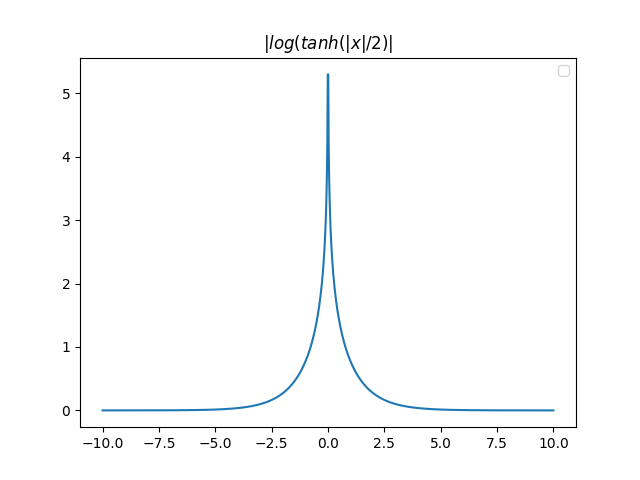
\includegraphics[width=\textwidth]{AWGN/logtanh.png}
		\end{figure}
\end{columns}
For a (3, 2) SPC code, 
\begin{gather*}
    \begin{split}
    f(l_{ext, 1}) & = f(l_2) + f(l_3) \\
    & = f(min(|l_2|, |l_3|))
    \end{split}
\end{gather*}
\begin{gather*}
    \begin{split}
    \Rightarrow |l_{ext, 1}| & = f^{-1}(f(min(|l_2|, |l_3|))) \\
    & = min(|l_2|, |l_3|)
    \end{split}
\end{gather*}
\end{frame}

\begin{frame}{Min-sum approximation for a (n, n-1) SPC code}
Generalising the previously discussed approximation, 
\begin{gather*}
    |l_{ext, n}| = min(|l_1|, |l_2|, ........, |l_{n-1}|)
\end{gather*}
To avoid the repeated computation of sgn() and the minima, we use the folowing procedure.
\begin{gather*}
    S = sgn(l(1) l(2) ....... l(n)) \\
    sgn(l_{ext, i}) = sgn(l_{i}) \times S \\
\end{gather*}
and
\begin{gather*}
    \text{Let }m_1 = min(|l_1|, |l_2|, ........, |l_n|) \\
    pos = argmin(|l_1|, |l_2|, ........, |l_n|) \\
    m_2 = min(|l_1|, |l_2|, ...., |l_{pos-1}|,  |l_{pos+1}|, ...., |l_n|)
\end{gather*}
\end{frame}

\subsection{Algorithm}
\begin{frame}{Decoding Algorithm}
    \begin{itemize}
        \item At $i^{th}$ zero-sum node, 
        \begin{itemize}
            \item Compute the parity $S_i = sgn(m_1)sgn(m_2)...sgn(m_{w_r-1})$.
            \item Compute the absolute value of LLR: 
            \begin{gather*}
                L_i = S_i \times \sum_{j = 1}^{w_r-1}\left|\log(\tanh\left|\frac{m_i}{2}\right|)\right|
            \end{gather*}
        \end{itemize}
        
        \item At $i^{th}$ repetition node, compute $$m_i = r_i + \sum_{j = 1}^{w_c-1} L_i$$
    \end{itemize}
    
Note that there is a slight abuse of notation; the indices 'j' denote the set of edges incident on the particular node.
\end{frame}

\subsection{Algorithm (with min-sum)}
\begin{frame}{Decoding Algorithm with min-sum approximation}
    \begin{itemize}
        \item At $i^{th}$ zero-sum node, 
        \begin{itemize}
            \item Compute the parity $S_i = sgn(m_1)sgn(m_2)...sgn(m_{w_r-1})$.
            \item Compute $pos = argmin(|m_1|, |m_2|, ........, |m_n|)$. \\~\\
                If $ i \neq pos, L_{i} = S_i \times |m_{pos}| $ \\~\\
                Else,  $ L_{i} = S_i \times min(|m_1|, |m_2|, ...., |m_{pos-1}|,  |m_{pos+1}|, ...., |m_n|) $
        \end{itemize}
        
        \item At $i^{th}$ repetition node, compute $$m_i = r_i + \sum_{j = 1}^{w_c-1} L_i$$
    \end{itemize}
    
Note that there is a slight abuse of notation; the indices 'j' denote the set of edges incident on the particular node.
\end{frame}

\subsection{Results}
\begin{frame}
\begin{block}{Terminal output for Belief Propagation}
    \begin{figure}
		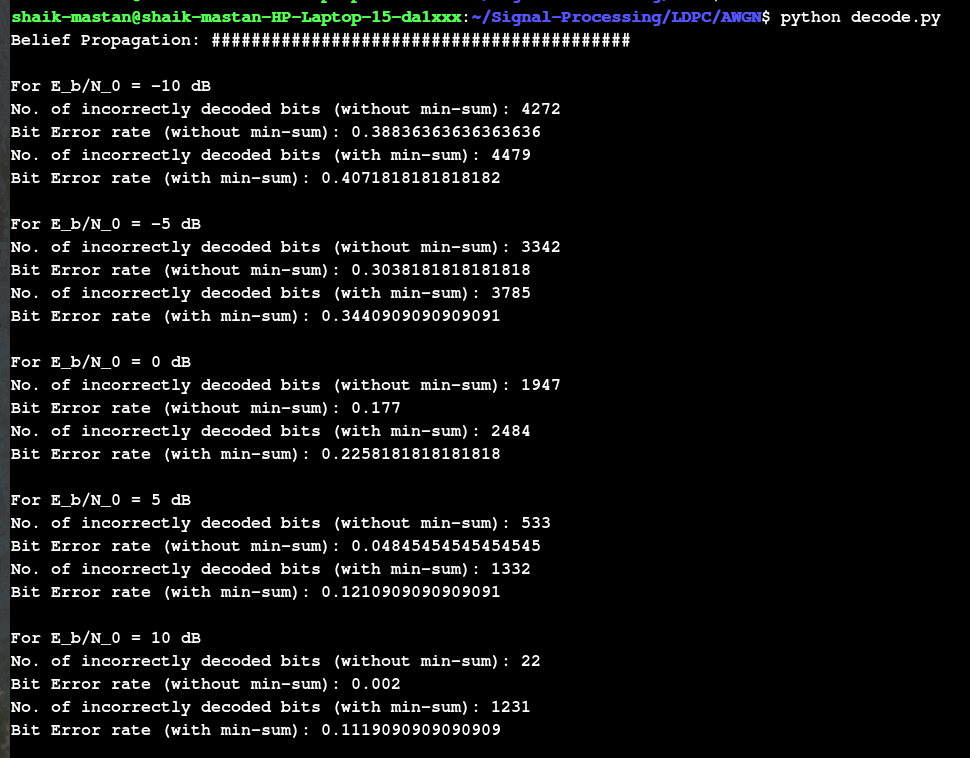
\includegraphics[width=0.8\textwidth]{AWGN/terminalAWGN_1.png}
	\end{figure}
\end{block}
\end{frame}

\begin{frame}
\begin{block}{Terminal output for Gallagher-A}
    \begin{figure}
		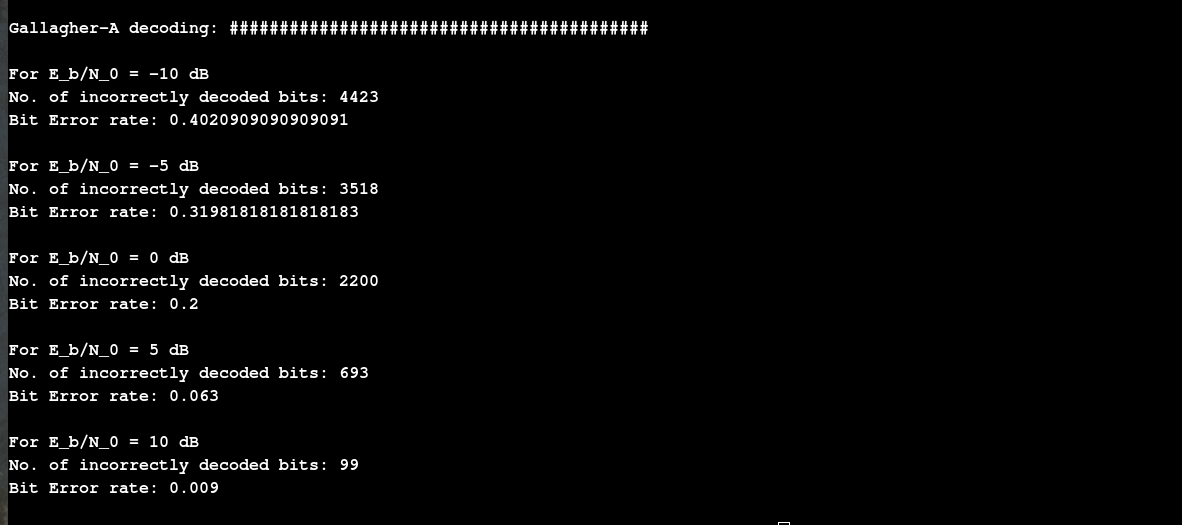
\includegraphics[width=\textwidth]{AWGN/terminalAWGN_2.png}
	\end{figure}
\end{block}

\end{frame}

\begin{frame}
\begin{block}{Comparison with different algorithms}
    \begin{figure}
		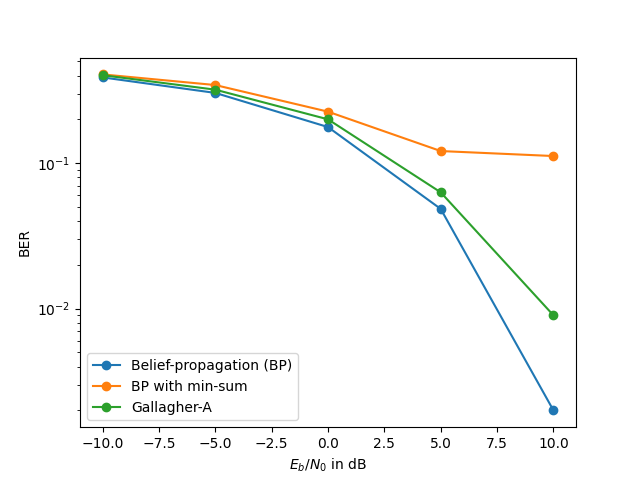
\includegraphics[width=0.8\textwidth]{AWGN/AWGN.png}
	\end{figure}
\end{block}

\end{frame}
\section{Binary Symmetric Channel}
\subsection{Gallagher-A decoder}
\begin{frame}{Gallagher’s Decoding Algorithm A}
\;\;\;\;\;\;Consider a ($d_v, d_c$) regular
LDPC code over the Binary Symmetric Channel (BSC). The BSC
is completely specified by a parameter p, the crossover probability.
The channel behaves as illustrated in below Figure. The correct bit is
transmitted with probability 1-p and a bit flip occurs with probability
p. Hence I = O = ±1. For this decoding algorithm $\mathcal{M}$ is also equal
to ±1. This is called hard-decision decoding 
\begin{exampleblock}{Binary Symmetric Channel}
\begin{figure}
			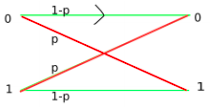
\includegraphics[width=8cm, height=4cm]{BSC/bsc.png}
			\label{bsc}
\end{figure}
\end{exampleblock}

\end{frame}

\begin{frame}{Gallagher's A (cont...)}
$\bullet$ $V^{0}(y) = y$  Variable nodes simply pass the received value as
their first message\\~\\
$\bullet$ $C^{(l)}(m_1, . . . , m_{d_c-1}) = m_1m_2 . . . m_{d_c-1}.$ For all l, the message from check node c to variable node v is the product of the messages received by c from all it’s neighbors except v. This makes perfect sense, since if the messages c received were indeed the correct values of the code word bit, then the parity check represented by c would only be satisfied if v were the product of the messages. Note that mod 2 addition corresponds
to multiplication after the identification of 0 with 1 and 1 with -1 respectively.\\~\\
$\bullet$ $V^{(l)}(y, m_1, . . . , m_{d_v-1}) = -y$ if all\;\; $ m_i = -y$ and y otherwise. For all subsequent rounds, v still sends the received value, y as its message to c unless there is unanimous agreement amongst all checks except c, that v participates in.
\end{frame}

\begin{frame}{Gallagher's A (cont...)}
\;\;\;\;\;\;\;\; This decoder is clearly sub-optimal since it does not even depend on the channel parameter p. Nonetheless, experimental simulations and theoretical analysis show that it is not too bad. We will analyze the asymptotic behavior of this decoder later in this section. in below Figures 
shows this algorithm in action. The code being used is a (3, 6) regular LDPC code. The all ones vector +\,+\,+\,+\,+\,+\,+\,+\,+\,+\, was transmitted. Due to channel noise, the received vector is +\,+\,+\,-\,+\,+\,+\,+\,+\,-\,. The first set of messages sent, Figure a, therefore correspond to the received values. The second set of messages, Figure b, were sent by the check nodes to the variable nodes. By 5 iterations, the algorithm converges to the vector -\,+\,-\,-\,-\,+\,-\,+\,+\,-\, which is indeed a valid code word but not the correct one. Hence this example serves to illustrate how message passing decoders can fail. Note that a high failure rate is expected since the block length is very small.\\~\\
following figures shows Gallagher’s algorithm A in action. R indicates the round number. The direction of arrows indicate the direction of message sent. Red corresponds to -1 and Green to 1    
\end{frame}
\begin{frame}{Gallagher's A (cont...)}
\begin{exampleblock}{Gallagher’s algorithm A in action}

\begin{figure}
			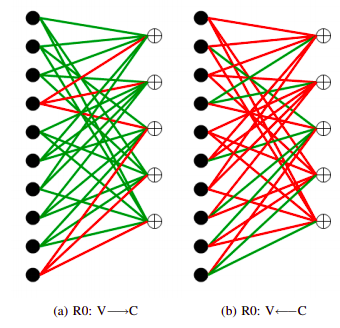
\includegraphics[width=6cm, height=3.3cm]{BSC/gallaghar fig 2a.png}
			\label{fig2a}
\end{figure}
\begin{figure}
			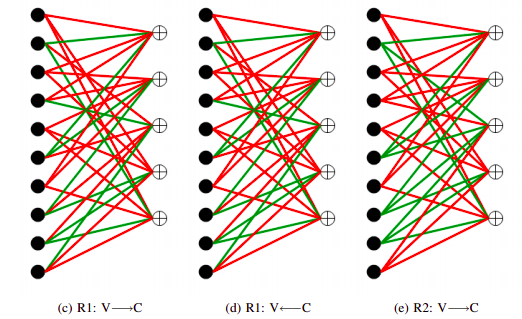
\includegraphics[width=8cm, height=3.3cm]{BSC/gallaghar fig 2b.png}
			\label{fig2b}
\end{figure}
\end{exampleblock}

\end{frame}

\subsection{Belief Propagation for BSC}
\begin{frame}{Belief Propagation for BSC}
$\bullet$ $V^{(0)}(y) = l_i$. Here $l_i$ is the log likelihood of the code word bit $x_i$ conditioned on the received bit $y_i$. The value depends on the channel model in use. For instance, consider the binary symmetric channel with crossover probability p. Then $y_i$ $\in$ \{-1, 1\}. Under the assumption of equiprobability, if the received code word was 1, then
 \begin{gather*}
     l_i = \log L(x_i/y_i = 1) = \log \frac{p}{1-p}
 \end{gather*} 
 otherwise 
 \begin{gather*}
     l_i = -\log\frac{p}{1-p}
 \end{gather*}

$\bullet$ $V^{(l)}(y, m_1, . . . , m_{d_v-1}) = l_i + $$\sum_{i=1}^{d_v-1} m_i$$ $ The reasoning behind this is that if $m_i$ are conditional log likelihoods of $x_i$, conditioned on independent random variables, then the
aggregate conditional would indeed by given by this equation
\end{frame}
\begin{frame}{Belief Propagation for BSC(cont...)}
\begin{gather*}
 C^{(l)}(m_1, . . . , m_{d_c-1})   = \log \frac{1 + \prod_{i=1}^{d_c-1} \tanh(m_i/2)}{1 - \prod_{i=1}^{d_c-1} \tanh(m_i/2)}
 \end{gather*}
$\bullet$  If the incoming messages are independent estimates of the log likelihood of $x_j$ , the neighbors of the check node computing the message excluding node xi, then the computed message $C^{(l)}$ correctly estimates the likelihood of $x_i$ conditioned on the the messages and the fact that the parity check represented by the check node is satisfied. \\~\\Consequently, under the independence assumption, the belief propagation algorithm correctly performs bit wise MAP decoding.
\end{frame}

\subsection{Results}
\begin{frame}
\begin{exampleblock}{Terminal output for Belief Propagation}
    \begin{figure}
		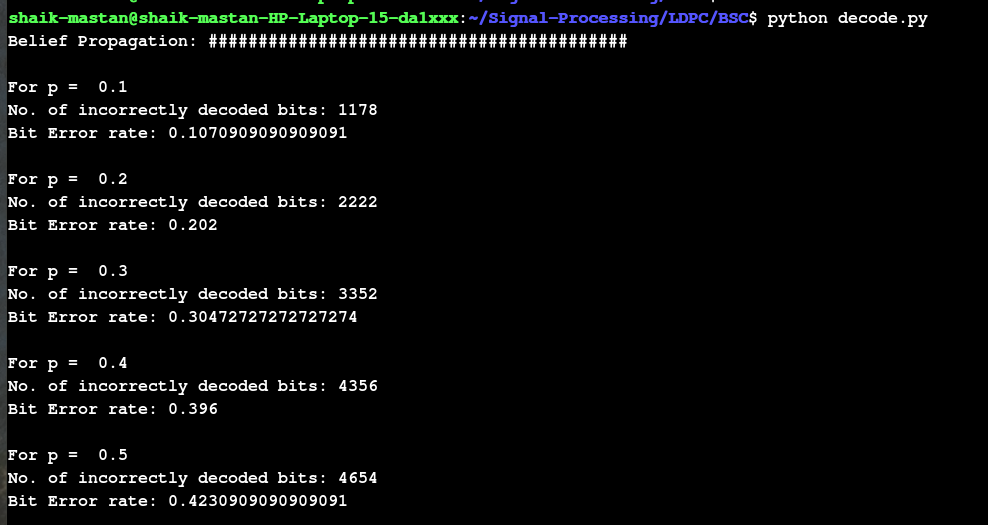
\includegraphics[width=\textwidth]{BSC/terminalBSC_1.png}
	\end{figure}
\end{exampleblock}
\end{frame}

\begin{frame}
\begin{exampleblock}{Terminal output for Gallagher-A}
    \begin{figure}
		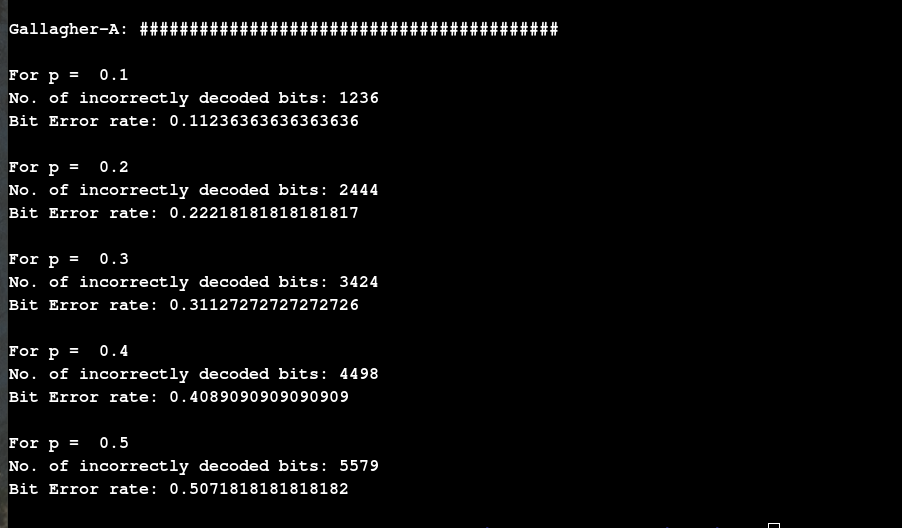
\includegraphics[width=\textwidth]{BSC/terminalBSC_2.png}
	\end{figure}
\end{exampleblock}
\end{frame}

\begin{frame}
\begin{exampleblock}{Comparison between the two decoders}
    \begin{figure}
		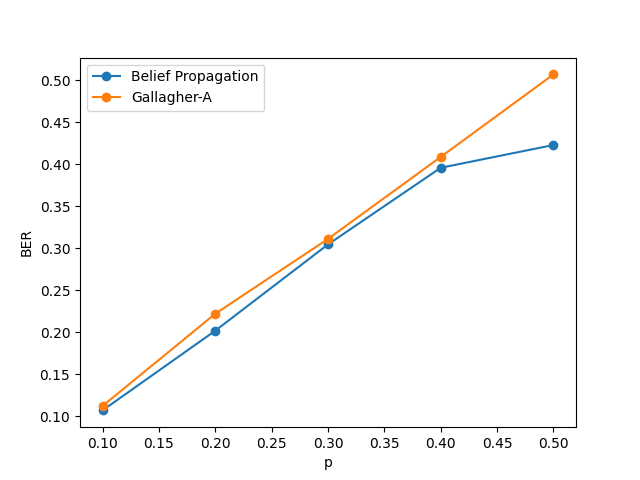
\includegraphics[width=0.9\textwidth]{BSC/BSC.png}
	\end{figure}
\end{exampleblock}

\end{frame}
\section{\textbf{Binary Erasure Channel}}
\subsection{Introduction}
\begin{frame}{Binary Erasure Channel(BEC)}
\;\;\;\;\;\;\;\;The binary erasure channel (BEC) models a memoryless channel with two inputs \{0, 1\} andthree outputs, \{0, 1, ?\}, where “?” is an “erasure symbol.” The probability that any transmitted
bit will be received correctly is 1 - p, that it will be erased is p, and that it will be received
incorrectly is zero. These transition probabilities are summarized in Figure  below.  
\begin{alertblock}{Transition probabilities of the binary erasure channel}
\begin{figure}
			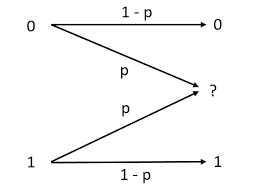
\includegraphics[width=6cm, height=3cm]{BEC/bec pic.png}
			\label{bec}
\end{figure}
\end{alertblock}
\end{frame}
\subsection{Iterative decoding of LDPC codes on the BEC}
\begin{frame}{Iterative decoding of LDPC codes on the BEC}
\;\;\;\;\;\;On the binary erasure channel, the sum-product algorithm is greatly simplified, because at any
time every variable corresponding to every edge in the code graph is either known perfectly
(unerased) or not known at all (erased). Iterative decoding using the sum-product algorithm
therefore reduces simply to the propagation of unerased variables through the code graph.\\~\\
\;\;\;\;\;\;There are only two types of nodes in a normal graph of an LDPC code repetition nodes and zero-sum nodes. If all variables are either correct or erased, then the
sum-product update rule for a repetition node reduces simply to:\\~\\
\;\;\;\;\;\;If any incident variable is unerased, then all other incident variables may be set equal to that variable, with complete confidence; otherwise, all incident variables remain erased.\\~\\
For a zero-sum node, the sum-product update rule reduces to:\\~\\
\;\;\;\;\;\;If all but one incident variable is unerased, then the remaining incident variable may
be set equal to the mod-2 sum of those inputs, with complete confidence; otherwise,
variable assignments remain unchanged.
\end{frame}
\begin{frame}{Iterative decoding of LDPC codes on the BEC(cont...)}
  Since all unerased variables are correct, there is no chance that these rules could produce a
variable assignment that conflicts with another assignment.\\~\\

\subsection{Results}
\begin{alertblock}{Terminal output}
   \begin{figure}
       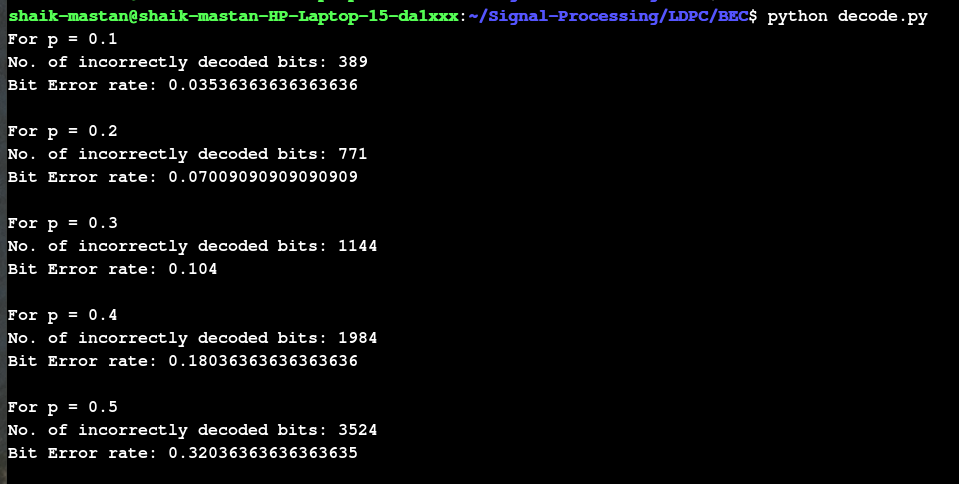
\includegraphics[width = 0.9\textwidth]{BEC/terminalBEC.png}
   \end{figure}
\end{alertblock}
\end{frame}

\begin{frame}
\begin{alertblock}{Plot}
   \begin{figure}
       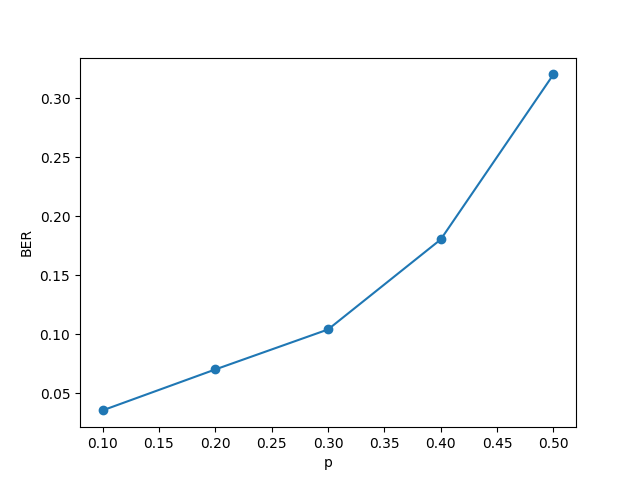
\includegraphics[width = 0.8\textwidth]{BEC/BEC.png}
   \end{figure}
  \end{alertblock}
\end{frame}

\begin{frame}
\noindent
{\color{purple} \rule{\linewidth}{0.5mm} }
\color{purple}
\Huge{\centerline{The End}}
\noindent
{\color{purple} \rule{\linewidth}{0.5mm} }
\end{frame}

\end{document}